\documentclass{article}

\usepackage{fancyhdr}
\usepackage{extramarks}
\usepackage{amsmath}
\usepackage{amsthm}
\usepackage{amsfonts}
\usepackage{tikz}
\usepackage[plain]{algorithm}
\usepackage{algpseudocode}

\usetikzlibrary{automata,positioning}

%
% Basic Document Settings
%

\topmargin=-0.45in
\evensidemargin=0in
\oddsidemargin=0in
\textwidth=6.5in
\textheight=9.0in
\headsep=0.25in

\linespread{2.0}

\pagestyle{fancy}
\lhead{\hmwkAuthorName}
\chead{\hmwkClass\ (\hmwkClassInstructor\ \hmwkClassTime)}
\rhead{\firstxmark}
\lfoot{\lastxmark}
\cfoot{\thepage}

\renewcommand\headrulewidth{0.4pt}
\renewcommand\footrulewidth{0.4pt}

\setlength\parindent{0pt}

%
% Create Problem Sections
%

\newcommand{\enterProblemHeader}[1]{
    \nobreak\extramarks{}{Problem \arabic{#1} continued on next page\ldots}\nobreak{}
    \nobreak\extramarks{Problem \arabic{#1} (continued)}{Problem \arabic{#1} continued on next page\ldots}\nobreak{}
}

\newcommand{\exitProblemHeader}[1]{
    \nobreak\extramarks{Problem \arabic{#1} (continued)}{Problem \arabic{#1} continued on next page\ldots}\nobreak{}
    \stepcounter{#1}
    \nobreak\extramarks{Problem \arabic{#1}}{}\nobreak{}
}

\setcounter{secnumdepth}{0}
\newcounter{partCounter}
\newcounter{homeworkProblemCounter}
\setcounter{homeworkProblemCounter}{1}
\nobreak\extramarks{Problem \arabic{homeworkProblemCounter}}{}\nobreak{}

%
% Homework Problem Environment
%
% This environment takes an optional argument. When given, it will adjust the
% problem counter. This is useful for when the problems given for your
% assignment aren't sequential. See the last 3 problems of this template for an
% example.
%
\newenvironment{homeworkProblem}[1][-1]{
    \ifnum#1>0
        \setcounter{homeworkProblemCounter}{#1}
    \fi
    \section{Problem \arabic{homeworkProblemCounter}}
    \setcounter{partCounter}{1}
    \enterProblemHeader{homeworkProblemCounter}
}{
    \exitProblemHeader{homeworkProblemCounter}
}

%
% Homework Details
%   - Title
%   - Due date
%   - Class
%   - Section/Time
%   - Instructor
%   - Author
%

\newcommand{\hmwkTitle}{Homework\ \#2}
\newcommand{\hmwkDueDate}{September 4th, 2014}
\newcommand{\hmwkClass}{Differential Equation}
\newcommand{\hmwkClassTime}{Section 061}
\newcommand{\hmwkClassInstructor}{Professor Heather Lee}
\newcommand{\hmwkAuthorName}{Yao Xiao}

%
% Title Page
%

\title{
    \vspace{2in}
    \textmd{\textbf{\hmwkClass:\ \hmwkTitle}}\\
    \normalsize\vspace{0.1in}\small{Due\ on\ \hmwkDueDate\ at 3:10pm}\\
    \vspace{0.1in}\large{\textit{\hmwkClassInstructor\ \hmwkClassTime}}
    \vspace{3in}
}

\author{\textbf{\hmwkAuthorName}}
\date{}

\renewcommand{\part}[1]{\textbf{\large Part \Alph{partCounter}}\stepcounter{partCounter}\\}

%
% Various Helper Commands
%

% Useful for algorithms
\newcommand{\alg}[1]{\textsc{\bfseries \footnotesize #1}}

% For derivatives
\newcommand{\deriv}[1]{\frac{\mathrm{d}}{\mathrm{d}x} (#1)}

% For partial derivatives
\newcommand{\pderiv}[2]{\frac{\partial}{\partial #1} (#2)}

% Integral dx
\newcommand{\dx}{\mathrm{d}x}

% Alias for the Solution section header
\newcommand{\solution}{\textbf{\large Solution}}

% Probability commands: Expectation, Variance, Covariance, Bias
\newcommand{\E}{\mathrm{E}}
\newcommand{\Var}{\mathrm{Var}}
\newcommand{\Cov}{\mathrm{Cov}}
\newcommand{\Bias}{\mathrm{Bias}}

\begin{document}

\maketitle

\pagebreak

\begin{homeworkProblem}
\(y'+y=te^{-t}+1 \) \\ \\
\textbf{Solution}

\begin{enumerate}



\item Field:\\ 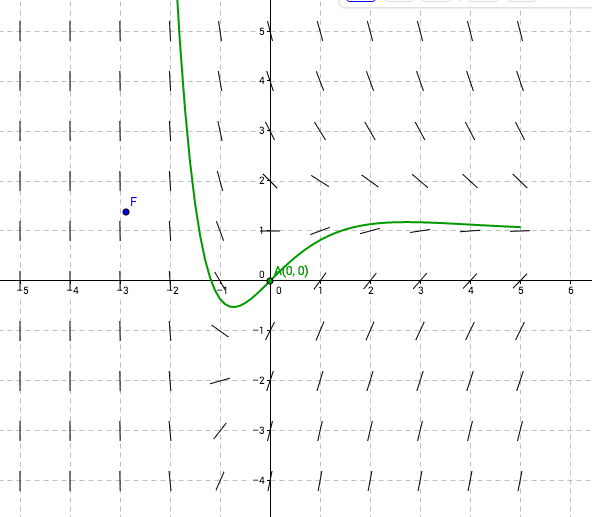
\includegraphics[scale=0.7]{image1.png} \\
\item When \( t>0 \) , since \(e^{-t} \to 0 \) so \(te^{-t}+1 \to 1\)
the solution will go towards \(1-y\)
\item  \[
		\begin{split}
		y'+y&=te^{-t}+1 \\				
		\mu(t) &= e^{t} \\		
		e^{t}y'+e^{t}y &=  t+e^{t}\\
		\frac{d(e^{t}y)}{dt} &= t+e^{t} \\
		\int \frac{d(e^{t}y)}{dt} &= \int t+e^{t}  \\
		e^{t}y &= \frac{1}{2}t^2+e^t+C \\
		y &=  \frac{1}{2}t^2e^{-t}+1+Ce^{-t}
		\end{split}		
\] \\
When \(t\to\infty\)  \(t^2e^{-t}\to 0\) \(e^{-t} \to 0\)
 \(y \to 1 \)


\end{enumerate}

\end{homeworkProblem}

\begin{homeworkProblem}
\(ty'+(t+1)y=2te^{-t}\)
\begin{enumerate}
\item Field:\\ 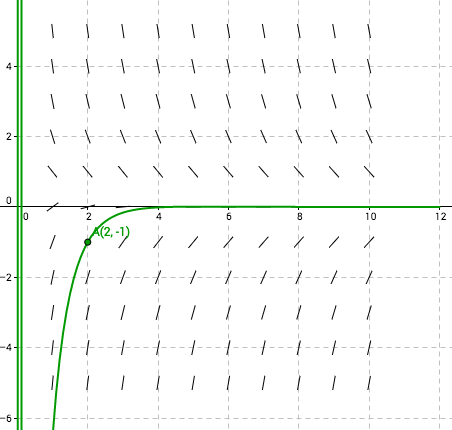
\includegraphics[scale=0.7]{image2.png}\\
As \(t\to0\) the solution will be either $\infty$ or $-\infty$ so the initial value do affect the result, \(a_0\) should close to 0
\item \[
	\begin{split}
			ty'+(t+1)y&=2te^{-t}\\
			y'+\frac{t+1}{t}y&=2e^{-t} \\
			\mu(t)=e^{t}t \\
			e^{t}ty'+e^{t}t\frac{t+1}{t}y&=2e^{-t}e^{t}t \\
			e^{t}ty'+e^{t}(t+1)y&=2t \\
			\frac{de^tty}{dt} &= 2t \\
			e^tty&=\int 2t\\
			e^tty&=t^2+C\\
			y&=\frac{t}{e^{t}}+\frac{C}{e^tt} \\
	\end{split}
\]
When \(y(1)=a\), \(\frac{1}{e}+\frac{C}{e}=\frac{1+C}{e}=a\)
Hence \(C=ae-1\) \\
\(y=\frac{t}{e^{t}}+\frac{ae-1}{e^tt} = \frac{t^2+ae-1}{e^tt} \)
As \(t\to 0\) , \(e^tt \to \infty\) \\
So \(ae-1\) changes the behavior, \(a_0=\frac{1}{e}\)
\item When \(a<\frac{1}{e}\) , As  \(t\to 0\) , \(y \to -\infty\) \\
When \(a=\frac{1}{e}\) , As  \(t\to 0\) , \(y =0\) \\
When \(a>\frac{1}{e}\) , As  \(t\to 0\) , \(y \to\infty\)
\end{enumerate}
\end{homeworkProblem}


\end{document}
